\documentclass{article}

% if you need to pass options to natbib, use, e.g.:
% \PassOptionsToPackage{numbers, compress}{natbib}
% before loading nips_2018

% ready for submission
\usepackage{nips_2018}

% to compile a preprint version, e.g., for submission to arXiv, add
% add the [preprint] option:
% \usepackage[preprint]{nips_2018}

% to compile a camera-ready version, add the [final] option, e.g.:
% \usepackage[final]{nips_2018}

% to avoid loading the natbib package, add option nonatbib:
% \usepackage[nonatbib]{nips_2018}

\usepackage[utf8]{inputenc} % allow utf-8 input
\usepackage[T1]{fontenc}    % use 8-bit T1 fonts
\usepackage{hyperref}       % hyperlinks
\usepackage{url}            % simple URL typesetting
\usepackage{booktabs}       % professional-quality tables
\usepackage{amsfonts}       % blackboard math symbols
\usepackage{nicefrac}       % compact symbols for 1/2, etc.
\usepackage{microtype}      % microtypography
\usepackage{graphicx} %package to manage images
\graphicspath{ {figures/} }
\usepackage{amsmath}
\usepackage{subfigure}

\title{Instance-sensitive Image Segmentation with Mask-RCNN and CRF}

% The \author macro works with any number of authors. There are two
% commands used to separate the names and addresses of multiple
% authors: \And and \AND.
%
% Using \And between authors leaves it to LaTeX to determine where to
% break the lines. Using \AND forces a line break at that point. So,
% if LaTeX puts 3 of 4 authors names on the first line, and the last
% on the second line, try using \AND instead of \And before the third
% author name.

\author{
  Haodong Zhou \\
  %% Department of Computer Science\\
  %% Cranberry-Lemon University\\
  %% Pittsburgh, PA 15213 \\
  %% \texttt{hippo@cs.cranberry-lemon.edu} \\
  %% examples of more authors
  \And
  Tzu-Chi Lin \\
  %% Affiliation \\
  %% Address \\
  %% \texttt{email} \\
  %% \AND
  %% Coauthor \\
  %% Affiliation \\
  %% Address \\
  %% \texttt{email} \\
  %% \And
  %% Coauthor \\
  %% Affiliation \\
  %% Address \\
  %% \texttt{email} \\
  %% \And
  %% Coauthor \\
  %% Affiliation \\
  %% Address \\
  %% \texttt{email} \\
}

\begin{document}
% \nipsfinalcopy is no longer used

\maketitle

\begin{abstract}

Image understanding problems such as object detection and semantic segmentation have made breakthroughs in recent years due to the development of deep learning techniques. We aim to provide a method to tackle with an instance segmentation problem that can be done in pixel level. Our model used Mask-RCNN incorporates with a conditional random field to further refine the result to the pixel level[4].

\end{abstract}

\section{Introduction}

Instance segmentation is one of a fundamental problem in computer vision that combines object detection and semantic segmentation. Semantic segmentation labels every pixel to its object class, without distinguishing different objects. Object detection does localize the object in a course, bounding-box level. These two problems are well-studied topics in scene understanding and have recently risen due to deep learning. The rising of autonomous driving and robotics industry also made this problem more important, since the accurate recognition is one of the main tasks in these two industries.

There are two different approaches to instance segmentation. First, based on object detection pipelines, where objects are first localized to different boxes, then applies the semantic segmentation method to further refine the object in each box. Another result is based on segment-based but rather box-based method. However, these methods do not consider the whole image, but rather independent proposals. Moreover, since they process numerous proposal independently, it is hard to produce segmentation maps of the image.

We provide a model which is based on the fully convolution neural network, and corporate the conditional random field to refine the result. Fully convolution neural network has been proved an efficient model to segmentation problem. We use CRF as a post-processing method, which has successfully pursued a joint learning method with CNN. We aim to use mean-field inference to convert the system into an end-to-end network, so we can use the convolutional layer as features to approximate CRF mean field inference.

\section{Related work}
Convolution Networks are driving advanced in segmentation. Traditional convolution networks solve for whole-image tasks like classification, and for local tasks like bounding box object detection. Because of the lack of the position information of the last layer in the network, it's hard to make a pixel level prediction of an image.

The fully convolutional network (FCN) trains an end-to-end, pixels-to-pixels network, which does a pixelwise prediction from supervised pre-trainning [4] . To improve the result of the convolution network, a conditional random field (CRF) is used to improve the marginal performance by Chen, L. C. et al [1]. Chen, L. C. [2, 3] claims the performance of semantic segmentation can be improved by using the atrous spatial pyramid pooling (ASPP) and using batch normalization within each ASPP. Also, an Encoder-Decoder with astrous convolution model was introduced to improve the performance. 

However, these works mainly focus on image semantic segmentation. For instance-sensitive segmentation, Dai, J. et al [5] proposed a method that uses different score map to distinguish different instance. Li, Y. et al [6] helps to improve the performance by training a region proposal network (RPN) in the model, which proposes region-of-interests on the score map for joint object segmentation and detection.


\section{Proposed approach}

\subsection{Pipeline}

Figure \ref{workflow} and \ref{workflow_image} shows a simple pipeline of our model. We aim to combine Mask-RCNN and CRF to get a refined result. Given an image as input, firstly we use Mask-RCNN to generate a bounding box and a mask for the image. Considering that the border of the mask is improvable, we use a Gaussian kernel to smooth the mask, which makes the border of the mask to be the state of "improvable" while keeps the center of the mask a high probability value.

The probability value generated by the smoothing kernel is then consider the unary potential of the CRF model. We further define the pairwise potential function as describe in section 3.3 and use mean field approximation to update maximum a posteriori probability (MAP) iteratively as described in section 3.4. 

\begin{figure}
  \centering
  %% \fbox{\rule[-.5cm]{0cm}{4cm} \rule[-.5cm]{4cm}{0cm}}
  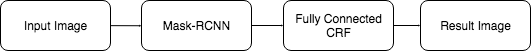
\includegraphics[width=14cm]{Workflow.png}
  \caption{Workflow of Instance Segmentation System}
  \label{workflow}
\end{figure}

\begin{figure}
  \centering
  %% \fbox{\rule[-.5cm]{0cm}{4cm} \rule[-.5cm]{4cm}{0cm}}
  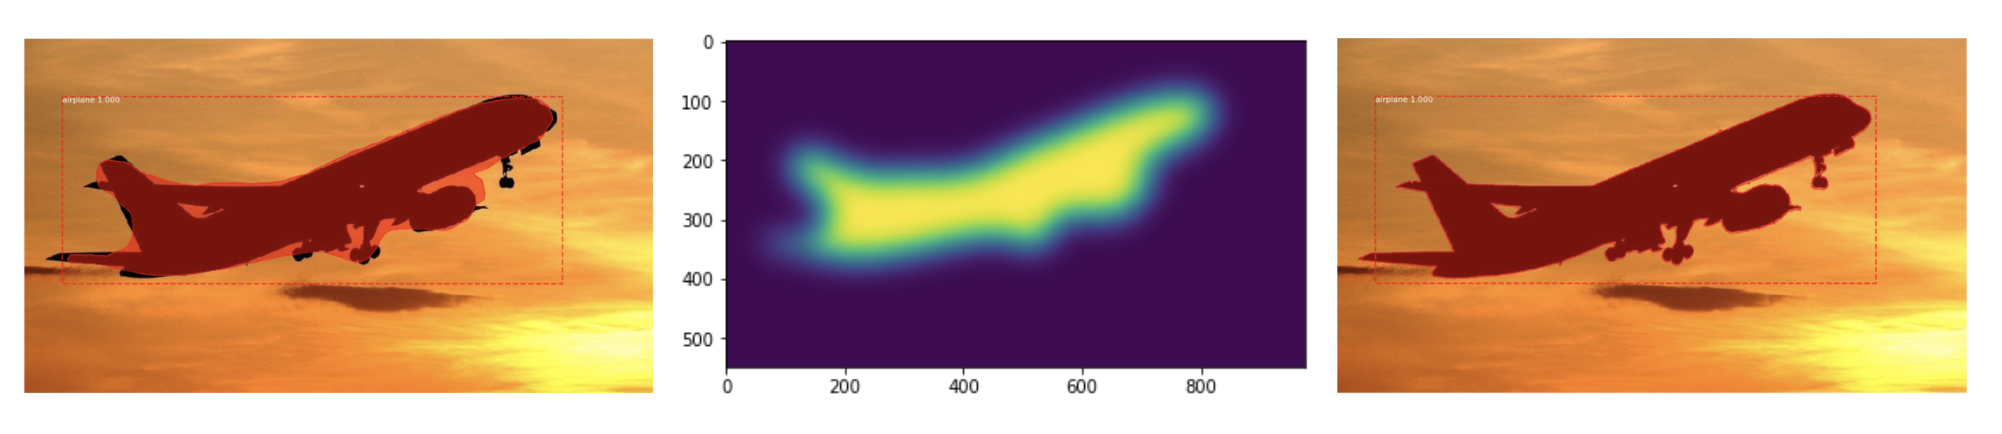
\includegraphics[width=14cm]{workflow.png}
  \caption{Left: result from Mask-RCNN. Middle: result generated by smoothing the mask, as the input to the CRF, which helps to improve the border performance. Right: result from the CRF refinement.}
  \label{workflow_image}
\end{figure}

\subsection{Mask-RCNN}

Mask-RCNN is a kind of network that achieve three functions: it can generate a bounding box, showing the position of the object, generate a class number and a possibility value indicating the type of the object and the probability, and the mask of the object. The Mask-rcnn shows a good result in the instance segmentation task.

The Faster-RCNN [8] is a network that can do multi-object detection and classification. The basic work flow of the Faster-RCNN is going through a CNN, using a RPN branch to generate ROIs(Region of Interest), sending the ROIs into a ROI Pooling layer and a classifier to get the bounding box and a classification result.

The Mask-RCNN [7] is based on the Faster-RCNN. It uses a FCN branch to generate the mask of the instance. Also, it uses the ROI Align layer instead of the ROI Pooling, which solves the problem caused by same feature size generated by different size ROIs. This will cause a low precision of the mask. Mask-RCNN is a instance sensitive segmentation, and it has the state-of-the-art result, which is used as a baseline in our project.


\subsection{Fully Connected Conditional Random Field Model}

We use the fully connected CRF model to further refine the result, which is shown in Figure \ref{fully_CRF}. We can see each pixel is represented by each node in CRF model. Consider a random field \textbf{X} defined over a set of variables $\{X_{1}, ..., X_{n}\}$ which ranges over possible pixel-level image labeling. Suppose there are k label, then the domain of each variable in X is a set of labels $L=\{l_{1},...l_{k}\}$. Consider another random field \textbf{I} defined over $\{I_{1}, ..., I_{n}\}$, which indicates the color vector of the pixel. 

\begin{figure}
  \centering
  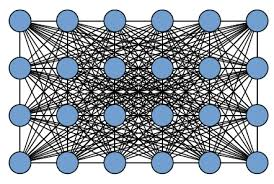
\includegraphics[width=0.5\textwidth]{denseCRF.jpeg}
  \caption{Example of fully connected CRF}
  \label{fully_CRF}
\end{figure}

Now we have two conditional random fields to consider, joint these two CRFs to get a new CRF (\textbf{X},\textbf{I}), which can be represented by Gibbs distribution $P(X|I)=\frac{1}{Z(I)}exp(-\sum\phi_{c}(X_{c}|I))$. Also, the Gibbs energy can be expressed as $E(x|I)=\sum\phi_{c}(x_{c}|I)$, which as our unary potential function in fully connected CRF. The maximum a-posterior (MAP) is $x^*=argmax_{x\in L^N}P(x|I)$, which is the distribution we want to compute.

The Gibbs energy in the fully connected CRF model can be represented as

\begin{center}
$E(x) = \sum_{i}{\psi_{u}(x_{i})}+\sum_{i\neq j}{\psi_{p}(x_{i}, x_{j})}$
\end{center}

The unary potential $\psi_{u}(x_{i})$ is computed independently for each pixel by mask-RCNN. Since the unary potential is produced independently, we could consider pairwise potential $\psi_{p}(x_{i}, x_{j})$ to make the image more consistent. The pairwise potential has the form

\begin{center}
$\psi_{p}(x_{i}, x_{j}) = \mu (x_{i},x_{j})\sum\limits_{m=1}^K w^{(m)}k^{(m)}(f_{i}, f_{j})$
\end{center}

where $\mu$ is the label compatibility function, $k^{(m)}(f_{i}, f_{j})$ is a Gaussian kernel and $w^{(m)}$ is its weight of linear combination. We could express the kernel function as two Gaussian kernel, considered in both color vectors and position 

\begin{center}
$k(f_{i},f_{j})=w^{(1)}exp(-\frac{\mid p_{i}-p_{j} \mid^{2}}{2\theta_{\alpha}^{2}}-\frac{\mid I_{i}-I_{j} \mid^{2}}{2\theta_{\beta}^{2}}) + w^{(2)}exp(-\frac{\mid p_{i}-p_{j} \mid^{2}}{2\theta_{\gamma}^{2}})$
\end{center}

where \textbf{I} indicates color vector and \textbf{p} is the position of the pixel. The first Gaussian kernel is called \textit{appearance kernel}, which is inspired by the nature of the object - nearby pixels with similar color are likely to be the same object. Later kernel is called \textit{smoothness kernel}, which aims to remove isolated region. 

\subsection{Mean Field Approximation}

The algorithm to compute MAP is based on the mean field approximation to the CRF distribution. We could see this approximation as a message passing algorithm and run it iteratively to get the approximation inference.

Assume the KL-divergence we want to compute is $D(Q||P)$. We can derive this Q as 

\begin{center}
$Q_{i}(x_{i}=l)=\frac{1}{z_{i}}exp\{-\psi_{\mu}(x_{i})-\sum_{l'\in L}\mu(l,l')\sum\limits_{m=1}^K w^{(m)}\sum_{j\neq i}k^{(m)}(f_{i},f_{j})Q_{j}(l')\}$
\end{center}

A detailed derivation is given in Appendix. We can decompose this formula into three steps. First, We can see $\sum\limits_{m=1}^K w^{(m)}\sum_{j\neq i}k^{(m)}(f_{i},f_{j})Q_{j}(l')$ as a message passing from all $X_{i}$ to $X_{j}$. $\sum_{l'\in L}\mu(l,l')$ is a compatibility transformation. And we update $exp\{-\psi_{\mu}(x_{i})-Q'\}$ locally at last step. 

For this message passing step, it takes quadratic time. We can improve this step to linear time by the observation this message passing step could be represented as a Gaussian filter in feature space [9]. We then only need to do a sampling and performs low-pass filter on this sample, which can be performed in O(N) time.

\section{Implementation Details}

Our project is based on the tensorflow. The Mask-RCNN part we used the implementation of the matterport, and the model is a pre-trained model \footnote{github.com/matterport/Mask\_RCNN/}, which already performs a good result. The output we get from the Mask-RCNN is a group of bounding box with a binary mask inside.

Then we apply CRF to masks one by one. We use a adaptive size Gaussian kernel to smooth the mask. Then the result will be sent into the CRF function. 

We adaptive our code to denseCRF code \footnote{github.com/lucasb-eyer/pydensecrf/}. Since we already have the unary potential from Mask-RCNN, we only have to create two Gaussian kernels for pairwise potential. There are some parameters we could tune on. For smoothness kernel parameter $\theta_{\gamma}$, it does not affect the result significantly. We just set $\theta_{\gamma}=1$ and found it work well. Unfortunately, the appearance kernel parameters $\theta_{\alpha}$ and $\theta_{\beta}$ cannot be computed effectively by gradient decent, since their gradient involves a sum of non-Gaussian kernels, which are not amenable to the same acceleration techniques. We simply use a grid search to find $\theta_{\alpha}$ and $\theta_{\beta}$.

After setting all the parameters in kernels, we need to run inference algorithm to compute MAP and assign each pixel by MAP. These steps could all be done by denseCRF API. Since we already found out 10 iterations may converge for KL-divergence as described in section 5.1, we set all other experiments to run 10 times iterations.


\section{Experiments}

\subsection{Convergence of mean field approximation}

We test the convergence of the mean field approximation first by analyzing KL-divergence between Q and P. Figure \ref{kl-divergence} shows the KL-divergence over iterations of the inference algorithm. We could see that it converges after 10 iterations. Hence, we set 10 as the number of iterations in all other experiments.

\begin{figure}
  \centering
  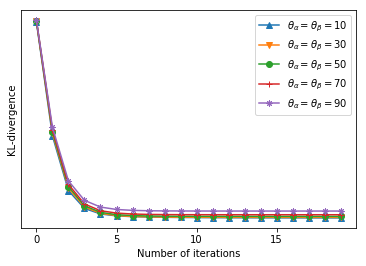
\includegraphics[width=0.6\textwidth]{kl_divergence.png}
  \caption{Convergence of KL-divergence}
  \label{kl-divergence}
\end{figure}

\begin{figure}
  \centering
  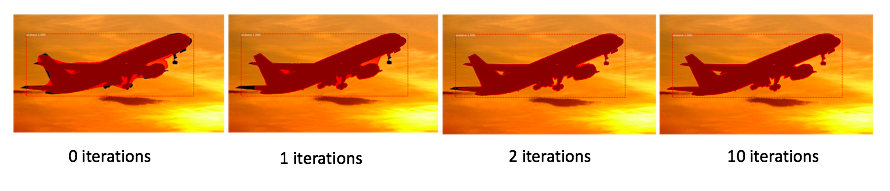
\includegraphics[width=14cm]{iteration.png}
  \caption{Iteration result of the image}
  \label{iteration_result}
\end{figure}  

\subsection{Grid search for parameters}

Figure \ref{grid_search_alpha} and \ref{grid_search_beta} shows a simple result for grid search of parameters $\theta_{\alpha}$ and $\theta_{\beta}$. We can see that for $\theta_{\alpha}=60$ and $\theta_{\beta}=10$ is good for our result. We then set $\theta_{\alpha}=60$ and $\theta_{\beta}=10$ to the following experiment.

\begin{figure}
    \centering
    \subfigure[$\theta_{\alpha}$=1]{
        \centering
        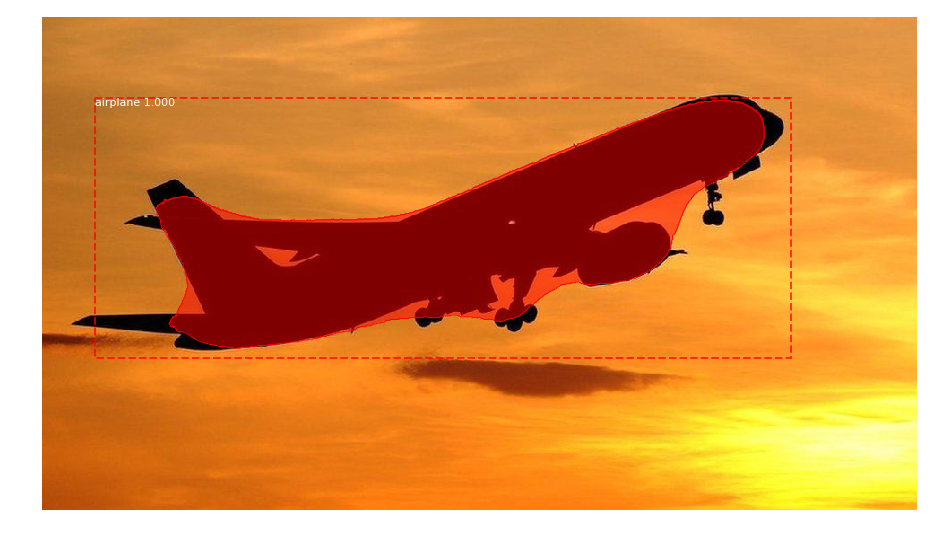
\includegraphics[width=0.18\textwidth]{./figures/alpha_1.png}
    }
    %
    \subfigure[$\theta_{\alpha}$=20]{
        \centering
        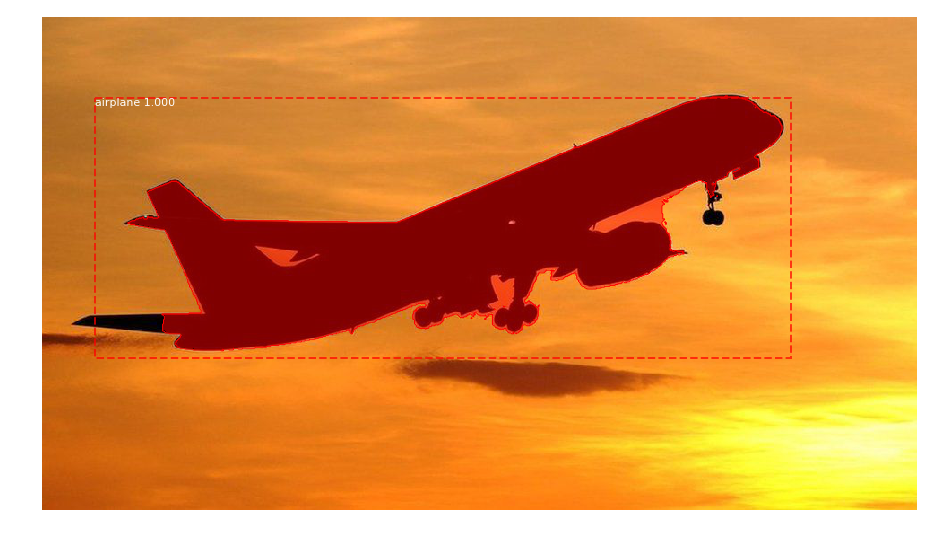
\includegraphics[width=0.18\textwidth]{./figures/alpha_20.png}
    }
    \subfigure[$\theta_{\alpha}$=40]{
        \centering
        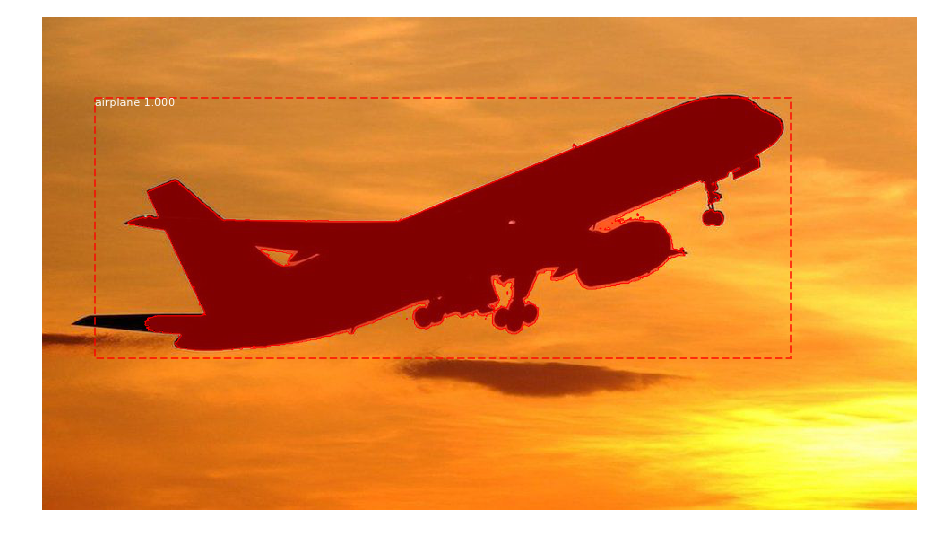
\includegraphics[width=0.18\textwidth]{./figures/alpha_40.png}
    }
    \subfigure[$\theta_{\alpha}$=60]{
        \centering
        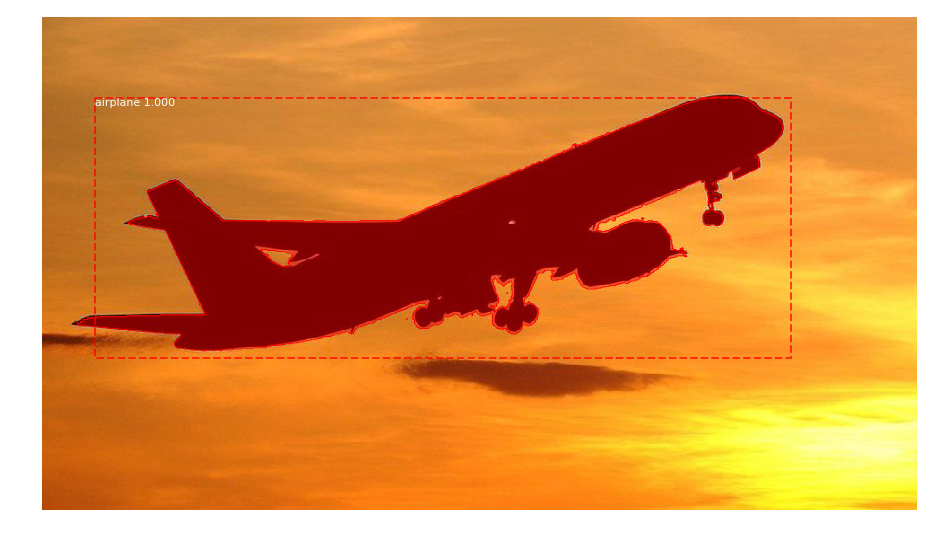
\includegraphics[width=0.18\textwidth]{./figures/alpha_60.png}
    }
    \subfigure[$\theta_{\alpha}$=80]{
        \centering
        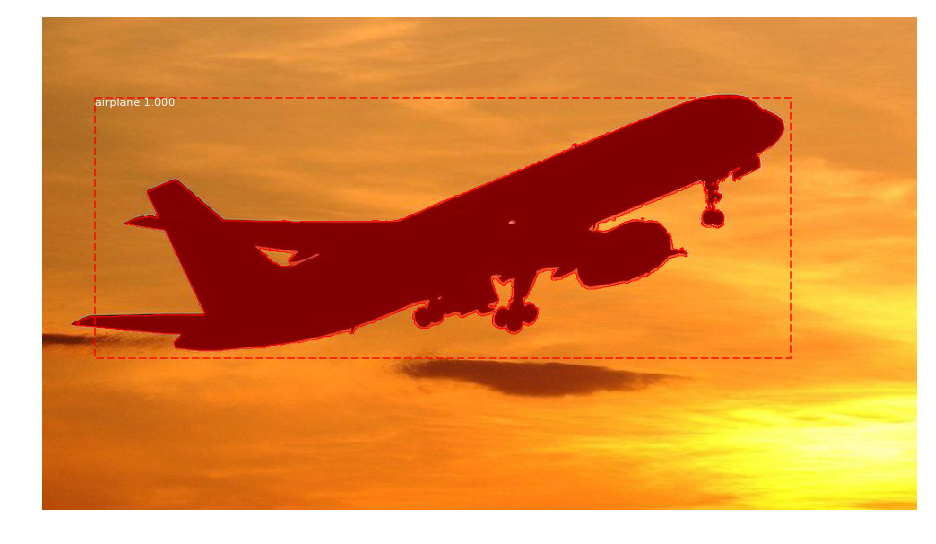
\includegraphics[width=0.18\textwidth]{./figures/alpha_80.png}
    }
    \caption{Grid search for $\theta_{\alpha}$}
    \label{grid_search_alpha}
\end{figure}

\begin{figure}
    \centering
    \subfigure[$\theta_{\beta}$=1]{
        \centering
        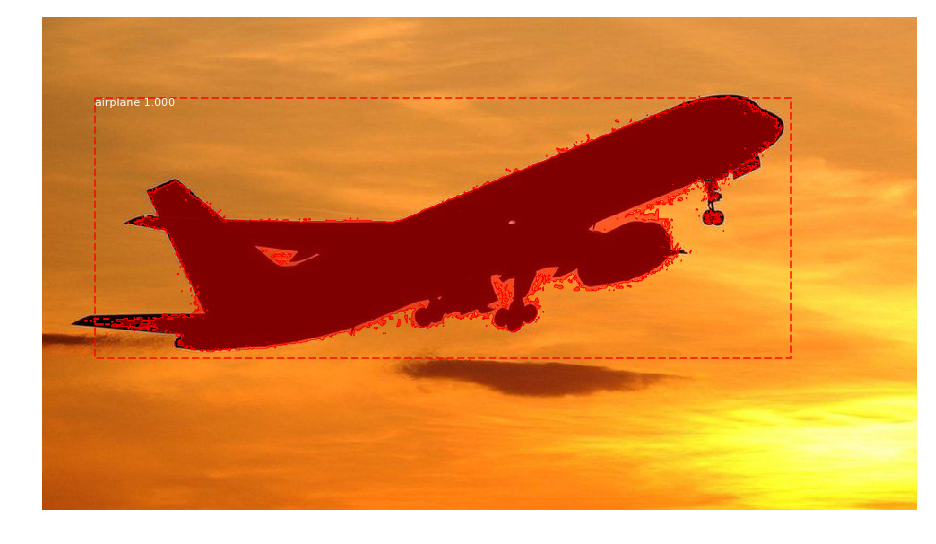
\includegraphics[width=0.18\textwidth]{./figures/beta_1.png}
    }
    %
    \subfigure[$\theta_{\beta}$=10]{
        \centering
        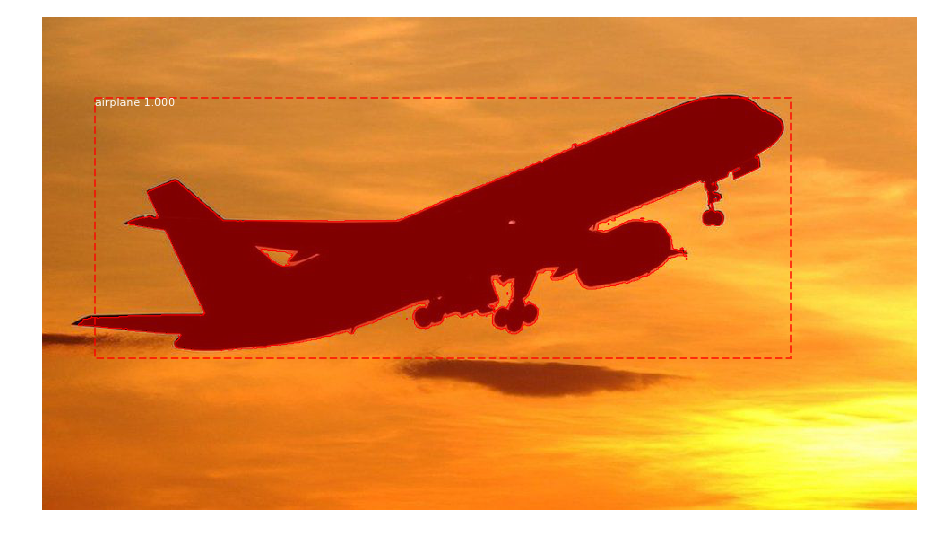
\includegraphics[width=0.18\textwidth]{./figures/beta_10.png}
    }
    \subfigure[$\theta_{\beta}$=20]{
        \centering
        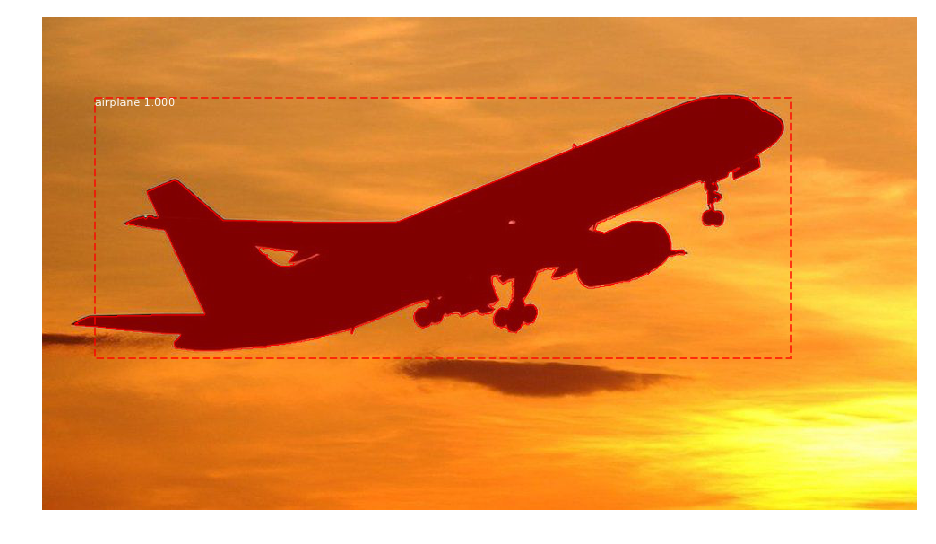
\includegraphics[width=0.18\textwidth]{./figures/beta_20.png}
    }
    \subfigure[$\theta_{\beta}$=30]{
        \centering
        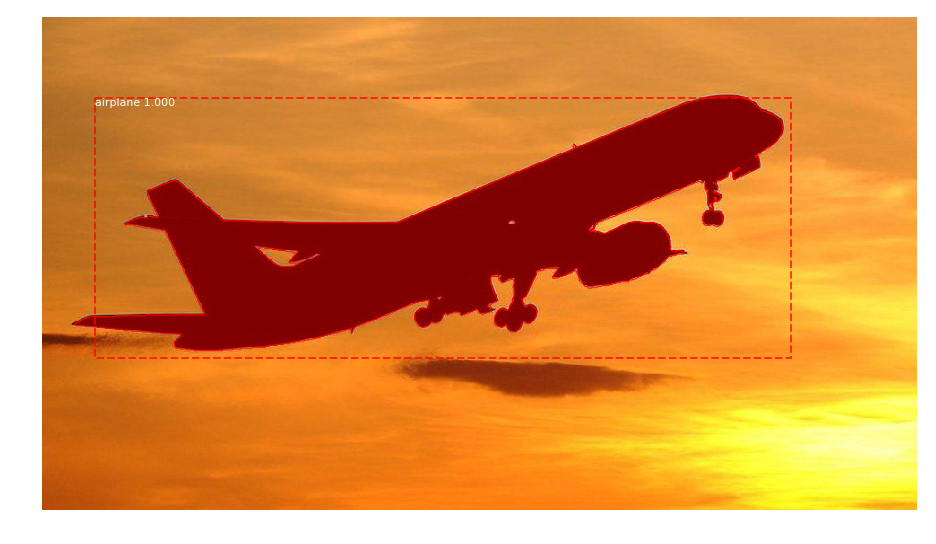
\includegraphics[width=0.18\textwidth]{./figures/beta_30.png}
    }
    \subfigure[$\theta_{\beta}$=40]{
        \centering
        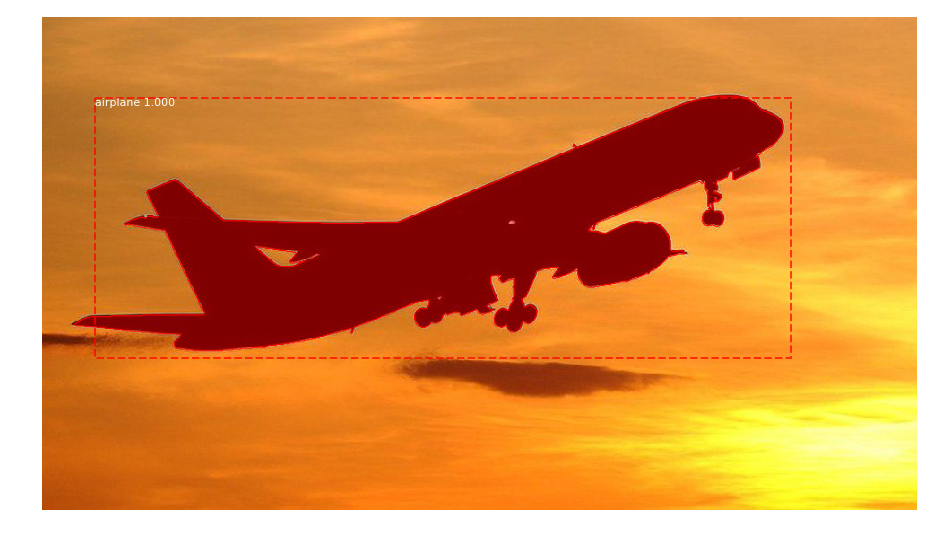
\includegraphics[width=0.18\textwidth]{./figures/beta_40.png}
    }
    \caption{Grid search for $\theta_{\beta}$}
    \label{grid_search_beta}
\end{figure}

\subsection{Evaluation method}
The performance is evaluated by intersection-over-union (IOU) between the predicted instances and the ground-truth instances. We report the standard COCO metrics including $AP$ (averaged over IoU thresholds), $AP_{50}$, $AP_{75}$ , and $AP_S$ , $AP_M$ , $AP_L$ (AP at different scales), which is the same method with the Mask-RCNN

\subsection{Result and Analysis}
The result based on the evaluation method is in the Table \ref{result-table}. Our result overall is similar with the result of the Mask R-CNN. Parameters is pretty hard to automatically adapt for each mask, and the current result is based on the parameters which makes small objects performs better than original Mask-RCNN. 

\begin{table}
  \caption{Instance Segmentation Result on COCO2014 Dataset}
  \label{result-table}
  \centering
  \begin{tabular}{ c | c c c | c c c } 
  \hline
  method & $AP$ & $AP_{50}$ & $AP_{75}$ & $AP_S$ & $AP_M$ & $AP_L$  \\ 
  \hline
  Mask R-CNN & 35.7 & 58.0 & 37.8 & 15.5 & 38.1 & 52.4 \\ 
  \hline
  Mask R-CNN with CRF & 35.2 & 58.7 & 36.4 & 17.3 & 36.5  & 49.8 \\ 
  \hline
  \end{tabular}
\end{table}

Some other results with specified tuned parameters are showed in the Figure \ref{e1}, \ref{e2} and \ref{e3} . We can find that after 10 iterations of CRF, the border of the mask is improved. However, to achieve these result, we increase the weight of the color, which causes that the part of the bird which has the similar color with the background color to has poor performance. 



\section{Future Work}

To further improve the performance, we may consider to put CRF model to end-to-end model so that we could jointly optimize the parameters of the CNN and the CRF, such as CRF as RNN model[10]. 

\section{Appendix}

\subsection{Detailed Derivation of Q}
We give a detailed derivation of Q in this section.

First we have Gibbs distribution of denseCRF

\begin{center}
$P(X) = \frac{1}{Z}P'(X) = \frac{1}{Z} exp(\sum_{i}{\psi_{u}(x_{i})}+\sum_{i\neq j}{\psi_{p}(x_{i}, x_{j})})$
\end{center}

We can derive KL-divergence as following


$D(Q||P)=\sum_{x}Q(x)log(\frac{Q(x)}{P(x)}) 
=-\sum_{x}Q(x)logP(x)+\sum Q(x)logQ(x)$ \\
$=-E_{X\in Q}[logP(X)]+E_{X\in Q}[logQ(x)]$ \\
$=-E_{X\in Q}[logP'(X)]+E_{X\in Q}[logZ]+\sum_{i}E_{X_{i}\in Q}[logQ_{i}(X_{i})]$ \\
$=-E_{X\in Q}[logP'(X)]+logZ+\sum_{i}E_{X_{i}\in Q_{i}}[logQ_{i}(X_{i})]$


Since our goal is to compute Q and $logZ$ do not have Q, we ignore this term.

At the same time, Q have to satisfy

\begin{center}
$\sum_{x_{i}}Q_{i}x_{i}=1$
\end{center}

By Lagrange Multiplier, we can get

\begin{center}
$L(Q_{i})=-E_{X\in Q}[logP'(X)]+\sum_{i}E_{X_{i}\in Q_{i}}[logQ_{i}(X_{i})]+\lambda (\sum_{x_{i}}Q_{i}(x_{i})-1)$
\end{center}

By partial differential we can get

\begin{center}
$\frac{\partial L(Q_{i})}{\partial Q_{i}(x_{i})}=-E_{\bar{X}\in Q_{i}}[logP'(X|x_{i})]-logQ_{i}(x_{i})-1+\lambda$
\end{center}

Set this to 0, we can get

\begin{center}
$Q_{i}(x_{i})=exp(\lambda -1)exp(-E_{\bar{X}\in Q_{i}}[logP'(X|x_{i})])$
\end{center}

We can see $exp(\lambda -1)$ as a constant number, so Q becomes

\begin{center}
$Q_{i}(x_{i})=\frac{1}{Z_{i}} exp(-E_{\bar{X}\in Q_{i}}[logP'(X|x_{i})])$
\end{center}
where Z is a normalization term.

We put $P'$ to this formula as we define at the beginning.

\begin{center}
$Q_{i}(x_{i})=\frac{1}{Z_{i}} exp(-E_{\bar{X}\in Q_{i}}[\sum_{i}{\psi_{u}(x_{i})}+\sum_{i\neq j}{\psi_{p}(x_{i}, x_{j})|x_{i}}])$
\end{center}

Since $x_{i}$ is known as label l, we now have

$Q_{i}(x_{i}=l)=\frac{1}{Z_{i}} exp(-\psi_{\mu}(l)-\sum_{j \neq i}E_{\bar{X}\in Q_{j}}\psi_{p}(l,X_{j}))$ \\
$= \frac{1}{Z_{i}} exp(-\psi_{\mu}(l)-\sum\limits_{m=1}^K w^{(m)}\sum\limits_{j \neq i}E_{X \in Q_{j}}[\mu(l,X_{j})k^{(m)}(f_{i},f_{j})])$ \\
$= \frac{1}{Z_{i}} exp(-\psi_{\mu}(l)-\sum\limits_{j\neq i}\sum\limits_{l'\in L} k^{(m)}(f_{i},f_{j})\mu(l,l')Q_{j}(l'))$ \\
$= \frac{1}{z_{i}}exp\{-\psi_{\mu}(x_{i})-\sum_{l'\in L}\mu(l,l')\sum\limits_{m=1}^K w^{(m)}\sum_{j\neq i}k^{(m)}(f_{i},f_{j})Q_{j}(l')\}$


where we can the result of 

\begin{center}
$Q_{i}(x_{i}=l)=\frac{1}{z_{i}}exp\{-\psi_{\mu}(x_{i})-\sum_{l'\in L}\mu(l,l')\sum\limits_{m=1}^K w^{(m)}\sum_{j\neq i}k^{(m)}(f_{i},f_{j})Q_{j}(l')\}$
\end{center}

\subsection{Contribution of each member}

Haodong Zhou is mainly responsible for Mask-RCNN, including its description in this paper and implementation of the code. Also, section 2 is written by him.

Tzu-Chi Lin is mainly responsible for CRF model, including its description in this paper and implementation of the code. Also, section 1 is written by him.

We together figure out how to combine Mask-RCNN and CRF together.

\section*{References}

\small

[1] Chen, L. C.,\  Papandreou, G.,\  Kokkinos, I.,\  Murphy, K.,\  
\& Yuille, A. L.\  (2018) Deeplab: Semantic image segmentation with deep convolutional nets, atrous convolution, and fully connected crfs. {\it IEEE transactions on pattern analysis and machine intelligence}, {\bf 40}(4),\  pp.834-848.

[2] Chen, L.C.,\  Papandreou, G.,\  Schroff, F.,\  \& Adam, H.\  (2017) Rethinking atrous convolution for semantic image segmentation. {\it arXiv preprint},  arXiv:1706.05587.

[3] Chen, L. C.,\  Zhu, Y.,\  Papandreou, G.,\  Schroff, F.,\  \& Adam, H. \ (2017) Encoder-decoder with atrous separable convolution for semantic image segmentation. {\it arXiv preprint} arXiv:1802.02611.

[4] Long, Jonathan,\ Evan Shelhamer,\  \& Trevor Darrell. \  (2015) Fully convolutional networks for semantic segmentation. {\it Proceedings of the IEEE conference on computer vision and pattern recognition} pp.3431-3440.

[5] Dai, J.,\  He, K.,\  Li, Y.,\  Ren, S.,\  \& Sun, J. (2016) Instance-sensitive fully convolutional networks. {\it European Conference on Computer Vision} pp. 534-549.

[6] Li, Y.,\  Qi, H.,\  Dai, J.,\  Ji, X.,\  \& Wei, Y.  (2016) Fully convolutional instance-aware semantic segmentation. {\it arXiv preprint} arXiv:1611.07709.

[7] He, K.,\  Gkioxari, G.,\  Dollár, P.\  \& Girshick, R.,\  2017, October. Mask r-cnn. {\it In Computer Vision (ICCV), 2017 IEEE International Conference on} (pp. 2980-2988). IEEE.

[8] Ren, S.,\  He, K.,\  Girshick, R.,\  \& Sun, J.,\  (2015). Faster r-cnn: Towards real-time object detection with region proposal networks. {\it In Advances in neural information processing systems} (pp. 91-99).

[9] Krahenbuhl, P.\ and Koltun, V.\ (2011) Efficient inference in fully connected crfs with gaussian edge potentials. In NIPS.

[10] Zheng, S.,\ Jayasumana, S., \ Romera-Paredes, B.,\ Vineet, V.,\ Su, Z.,\ Du, D.,\ Huang, C.,\ and Torr, P.\ (2015) Conditional random fields as recurrent neural networks, in IEEE ICCV.

\begin{figure}
  \centering
  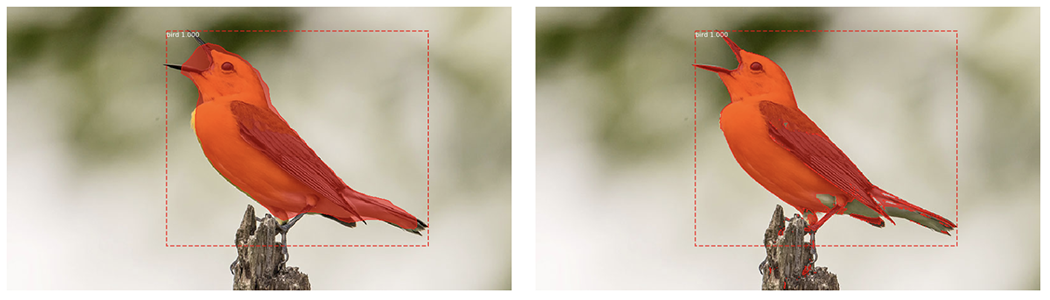
\includegraphics[width=14cm]{e1.png}
  \caption{Example With Tuned Parameters}
  \label{e1}
\end{figure}  

\begin{figure}
  \centering
  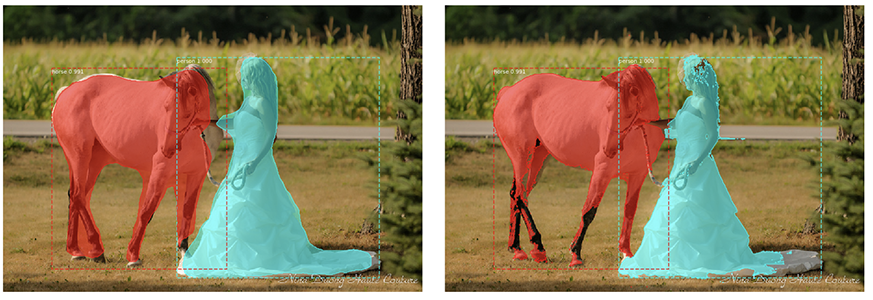
\includegraphics[width=14cm]{e2.png}
  \caption{Example With Tuned Parameters}
  \label{e2}
\end{figure}  

\begin{figure}
  \centering
  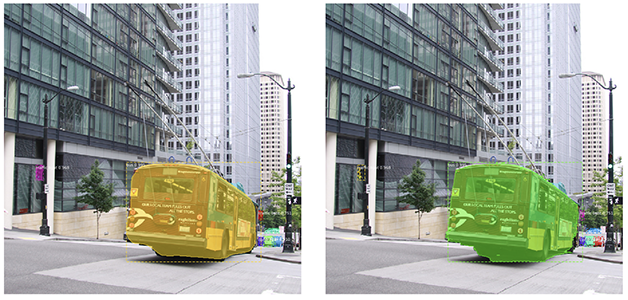
\includegraphics[width=14cm]{e3.png}
  \caption{Example With Tuned Parameters}
  \label{e3}
\end{figure}  

\end{document}
